\chapter{Introduction}\label{Chp:ref:introduction}
Our task in the inversion\index{inversion} is to find the geological structure within a given three-dimensional region $\Omega$ from given geophysical 
observations\index{observation}. 
The structure is described by a \emph{level set function} $m$\index{level set function}.
This function can be a scalar function or may have several components,
see Chapter~\ref{Chp:ref:regularization} for more details.
Its values are dimensionless and should be between zero and one.
However, the latter condition is not enforced.
Through a mapping (see Chapter~\ref{Chp:ref:mapping}\index{mapping}) the values
of the level set function are mapped onto physical parameter $p^f$\index{physical parameter}.
The physical parameter feeds into one or more forward models\index{forward model}
which return a prediction for the observations, see Chapter~\ref{Chp:ref:forward models}.
An inversion may consider several forward models at once which we call
\emph{joint inversion}\index{joint inversion}.


The level set function describing the actual geological structure is given as
the function which minimizes a particular \emph{cost function}
$J$\index{cost function}.
This cost function is a composition of the difference of the predicted
observations to the actual observations for the relevant forward models, and
the regularization term\index{regularization} which controls the smoothness of
the level set function.
In general the cost function $J$ takes the form
\begin{equation}\label{REF:EQU:INTRO 1}
J(m) = J^{reg}(m) + \sum_{f} \mu^{data}_{f} \cdot J^{f}(p^f)
\end{equation} 
where $J^{f}(p)$ is a measure of the defect of the observations predicted for
the parameter $p^f$ against the observations for forward model $f$, and
$J^{reg}(m)$ is the regularization term.
The weighting factors $\mu^{data}_{f}$ are dimensionless, non-negative
trade-off factors\index{trade-off factor}.
Potentially, values for the trade-off factors are altered during the inversion
process in order to improve the balance between the regularization term and
the data defect terms\footnote{The current version does not support an automated selection 
of trade-off factors}.
The physical parameter $p^f$ depends on the level set function
$m$ in a known form:
\begin{equation}\label{REF:EQU:INTRO 1b}
p^f = M_{f}(m)
\end{equation} 
where $M_f$ is a given mapping. For the case of gravity inversion
the $M_f$ is a simple linear function mapping the level set function $m$ with dimensionless values 
to physical density anomaly values $\rho$.
(see Chapter~\ref{Chp:ref:mapping}\index{mapping}). In its simplest from the mapping is given as 
$\rho = \rho_0 \cdot m$ where $\rho_0$ is a reference density. It is pointed out that 
the inversion techniques applied do not constrain limits to the values of the level set function
although there is the notion that its values are between zero and one. However, 
limits can be enforced to physical parameters using appropriate mappings.

The level set function $m$ and consequently the physical parameters $p^f$ are 
defined over a three dimensional domain $\Omega$ which represented by an \escript 
\class{Domain} object, see \cite{ESCRIPT}. The domain builder methods provide 
functions to build appropriate domains from field data sets, see Section~\ref{Chp:ref:domain builder}.
In general the domain is a rectangular three-dimensional domain where the third dimension $x_2=z$ represents
depth. The $z=0$ surface defines the surface of the earth where $z<0$ is defining the subsurface region and
$z>0$ is defining the region above the surface, see Figure~\ref{fig:cartesianDomain}. In general physical parameters such as
density and susceptibility anomaly are known above the surface, typically assumed to be zero. 
For subregions where a physical parameter is known it is assumed that the corresponding level set function as 
the value zero. If required, non-zero values for the physical parameters can be set using appropriate mapping.      

\section{Cartesian Domain}
For the Cartesian domain\index{Cartesian Domain} $\Omega$ we assume a flat Earth in the form
\begin{equation} \label{REF:EQU:INTRO 8}
\Omega = [x^{min}_0, x^{max}_0] \times
 [x^{min}_1, x^{max}_1] \times
 [x^{min}_2, x^{max}_2] 
\end{equation} 
and use the Universal Transverse Mercator (UTM) coordinate system\footnote{See
    e.g. \url{http://en.wikipedia.org/wiki/Universal_Transverse_Mercator_coordinate_system}.}
where $x_0$ represents the easting, $x_1$ the northing and $x_2$ the altitude.
In this way, all three coordinates can be given in meters with minimal
distortion when visualizing the domain.
The origin in vertical direction (altitude 0) corresponds to sea level.
A proper inversion set up requires a buffer zone in all dimensions.
Figure~\ref{fig:cartesianDomain} depicts these as areas shaded in red (padding
area) and blue (air buffer).
While the inversion results contain values for the entire domain the buffer zone
should be disregarded when performing any analysis.
In other words, only the region labeled \emph{data area} in
Figure~\ref{fig:cartesianDomain} contains useful information.
Both the thickness of the air layer and the amount of padding in the $x_0$/$x_1$
dimension is configurable when setting up an inversion.

\begin{figure}[ht]
    \centering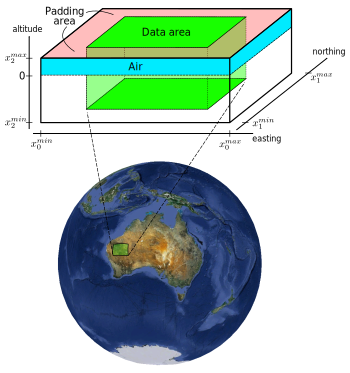
\includegraphics{cartesian}
    \caption{Illustration of domain extents, mapping and padding area}
    \label{fig:cartesianDomain}
\end{figure}

\begin{equation}\label{REF:EQU:INTRO 9}
\begin{array}{rcl}
Q_0  & = &  Q_{\phi} \\
Q_1  & = & -Q_{\theta} \\
Q_2  & = & -Q_r \\
\end{array}
\end{equation}

\section{Sphere Shell Segment}
This is not supported yet.

The regularization cost function $J^{reg}$ is given through a cost function
kernel\index{cost function!kernel} $K^{reg}$ in the form
\begin{equation}\label{REF:EQU:INTRO 2a}
J^{reg}(m) = \int_{\Omega} K^{reg}(m, \nabla m) \; dx
\end{equation} 
where $\Omega$ is the region of interest. $K^{reg}$ is a given function of the
level set function $m$ and its gradient $\nabla m$.
In case of a multi-component level set function the kernel may consider cross
correlation terms between the components.
Similar for the data defect for forward model $f$ we use a cost function kernel $K^{f}$ 
\begin{equation}\label{REF:EQU:INTRO 2b}
J^{f}(p^f) = \int_{\Omega} K^{f}(u^f, \nabla u^f,p^f) \; dx
\end{equation} 
where $u_f$ is a solution of a partial differential equation (PDE) involving
the physical parameter $p^f$.
The cost function kernel may directly depend on $u^f$, its gradient
$\nabla u^f$ and the physical parameter $p^f$.





 
